\documentclass[a4paper,11pt]{report}
\usepackage[showexo=true,showcorr=false,showdegree=true]{../packages/coursclassed}
%Commenter ou enlever le commentaire sur la ligne suivante pour montrer le niveau
\toggletrue{montrerNiveaux}
%permet de gérer l'espacement entre les items des env enumerate et enumitem
\usepackage{enumitem}
\setlist[enumerate]{align=left,leftmargin=1cm,itemsep=10pt,parsep=0pt,topsep=0pt,rightmargin=0.5cm}
\setlist[itemize]{align=left,labelsep=1em,leftmargin=*,itemsep=0pt,parsep=0pt,topsep=0pt,rightmargin=0cm}
%permet de gerer l'espacement entre les colonnes de multicols
\setlength\columnsep{35pt}

\usepackage{numprint}

\begin{document}

%%%%%%%%%%%%%%%%% À MODIFIER POUR CHAQUE SERIE %%%%%%%%%%%%%%%%%%%%%%%%%%%%%
\newcommand{\chapterName}{Fonctions et algèbre}
\newcommand{\serieName}{Proportionnalité : Pente}

%%%%%%%%%%%%%%%%%% PREMIERE PAGE NE PAS MODIFER %%%%%%%%%%%%%%%%%%%%%%%%
% le chapitre en cours, ne pas changer au cours d'une série
\chapter*{\chapterName}
\thispagestyle{empty}

%%%%% LISTE AIDE MEMOIRE %%%%%%
\begin{amL}{\serieName}{
\item Proportionnalité - Généralités (page 55)
\item Résoudre un problème de proportionnalité (page 57)
\item Pente (page 60)
\item Déterminer la pente moyenne (page 60)
}\end{amL}

%%%%%%%%%%%%%%% DEBUT DE LA SERIE NE PAS MODIFIER %%%%%%%%%%%%%%%%%%%%%%%%%%%%%
\section*{\serieName}
\setcounter{page}{1}

%%%%%%%%%%% LES EXERCICES %%%%%%%%%%%%%%%%%%%%%%%%%%%%%%%%%%%%


\begin{exol}{FA72}{87}{1} %panneau pente
\end{exol}

\begin{resolu}{Calculer la pente d'une droite}{
Calcule la pente de chacune des droites. Exprime ton résultat en fraction irréductible et en $\%$.
\begin{tasks}(2)
    \task ~\\
    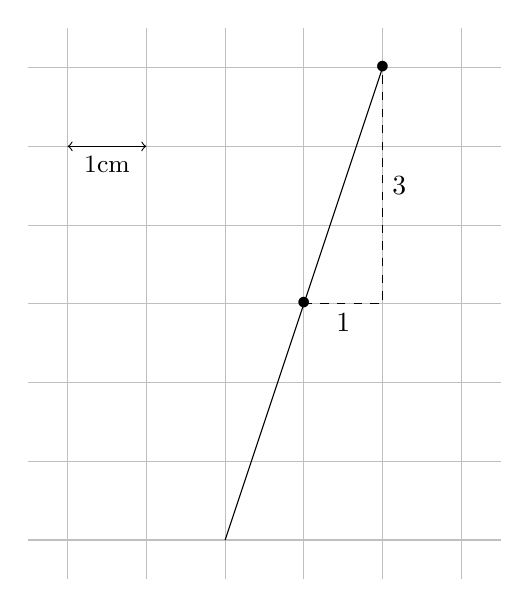
\begin{tikzpicture}
        \draw[color=gray!50] (-0.5,-0.5) grid[step=1] (5.5,6.5) ;
        \draw[<->] (0,5) -- node[below] {{\small \tunit{1}{cm}}} (1,5) ;
        \draw (2,0) -- (4,6) ;
        %\node at (2,0) {$\bullet$} ;
        \node at (3,3) {$\bullet$} ;
        \node at (4,6) {$\bullet$} ;
        \draw[dashed] (3,3) --node[below] {$1$} (4,3) --node[right] {3} (4,6) ;
    \end{tikzpicture}

    \begin{align*}
        \textrm{pente}&=\dfrac{\textrm{distance verticale}}{\textrm{distance horizontale}} \\
        &=\dfrac{3}{1} \\
        &=300\%
    \end{align*}

    \task ~\\
    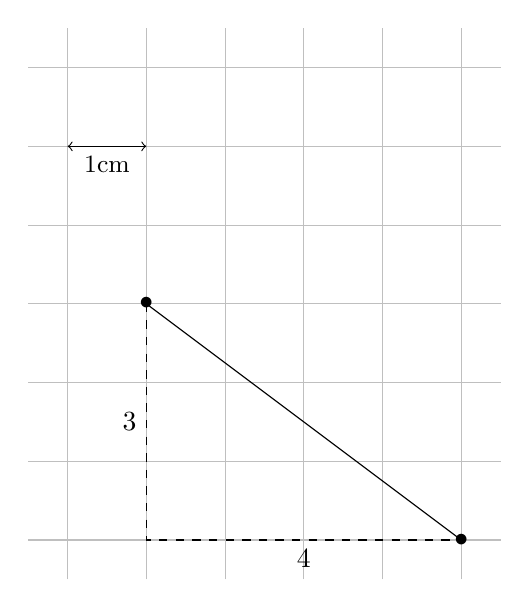
\begin{tikzpicture}
        \draw[color=gray!50] (-0.5,-0.5) grid[step=1] (5.5,6.5) ;
        \draw[<->] (0,5) -- node[below] {{\small \tunit{1}{cm}}} (1,5) ;
        \draw (1,3) -- (5,0) ;
        \node at (1,3) {$\bullet$} ;
        \node at (5,0) {$\bullet$} ;
        \draw[dashed] (1,3) --node[left] {$3$} (1,0) --node[below] {$4$} (5,0) ;
    \end{tikzpicture}

    \begin{align*}
        \textrm{pente}&=\dfrac{\textrm{distance verticale}}{\textrm{distance horizontale}} \\
        &=\dfrac{-3}{4} \\
        &=-75\%
    \end{align*}
    
\end{tasks}
}{1}
\end{resolu}


\begin{exop}{
Calcule la pente de chacune des droites. Exprime ton résultat en fraction irréductible.
\begin{tasks}(2)
    \task ~\\
    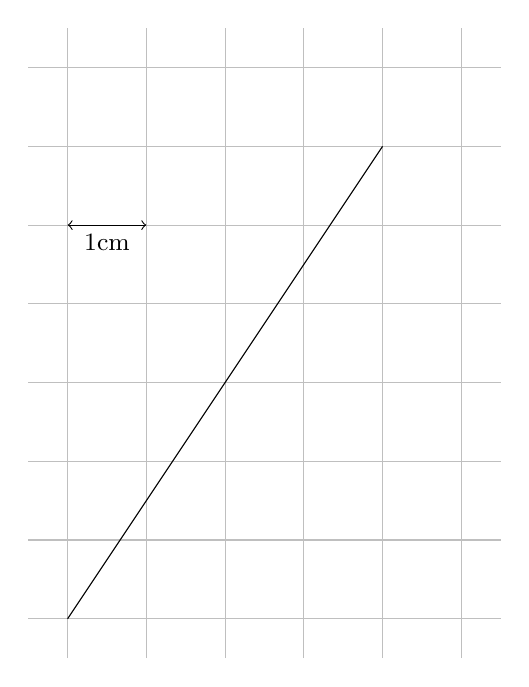
\begin{tikzpicture}
        \draw[color=gray!50] (-0.5,-0.5) grid[step=1] (5.5,7.5) ;
        \draw[<->] (0,5) -- node[below] {{\small \tunit{1}{cm}}} (1,5) ;
        \draw (0,0) -- (4,6) ;
    \end{tikzpicture}

    \task ~\\
    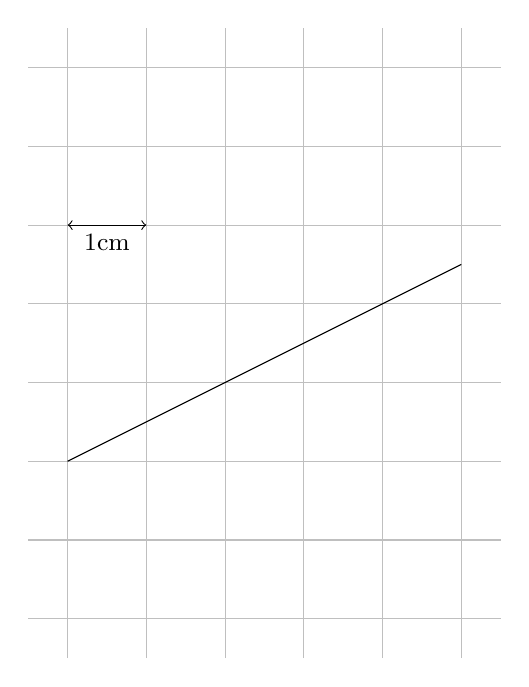
\begin{tikzpicture}
        \draw[color=gray!50] (-0.5,-0.5) grid[step=1] (5.5,7.5) ;
        \draw[<->] (0,5) -- node[below] {{\small \tunit{1}{cm}}} (1,5) ;
        \draw (0,2) -- (5,4.5) ;
    \end{tikzpicture}

    \task ~\\
    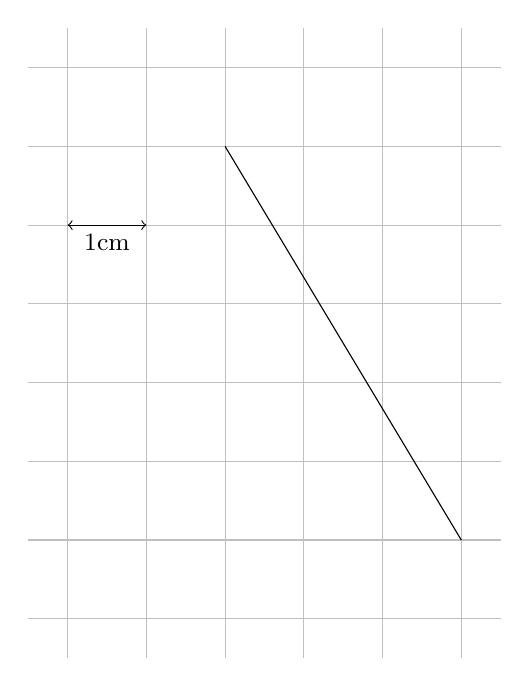
\begin{tikzpicture}
        \draw[color=gray!50] (-0.5,-0.5) grid[step=1] (5.5,7.5) ;
        \draw[<->] (0,5) -- node[below] {{\small \tunit{1}{cm}}} (1,5) ;
        \draw (2,6) -- (5,1) ;
    \end{tikzpicture}

    \task ~\\
    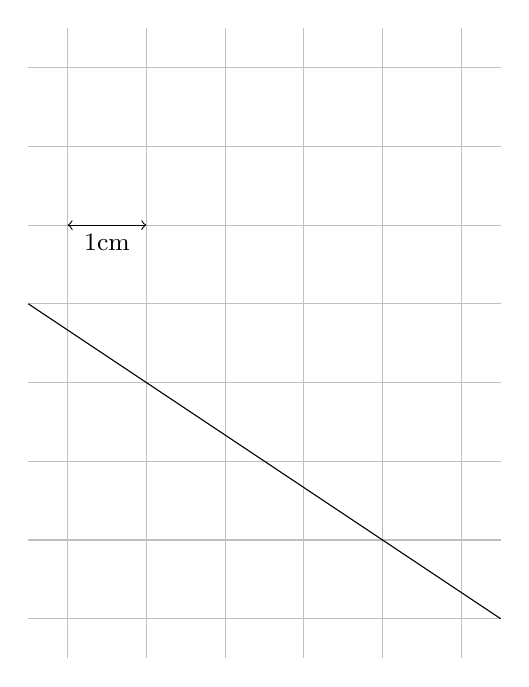
\begin{tikzpicture}
        \draw[color=gray!50] (-0.5,-0.5) grid[step=1] (5.5,7.5) ;
        \draw[<->] (0,5) -- node[below] {{\small \tunit{1}{cm}}} (1,5) ;
        \draw (-0.5,4) -- (5.5,0) ;
    \end{tikzpicture}
    
\end{tasks}
}{1}    
\end{exop}


\begin{exop}{
Calcule la pente de chacune des droites. Exprime ton résultat en $\%$.
\begin{tasks}(2)
    \task ~\\
    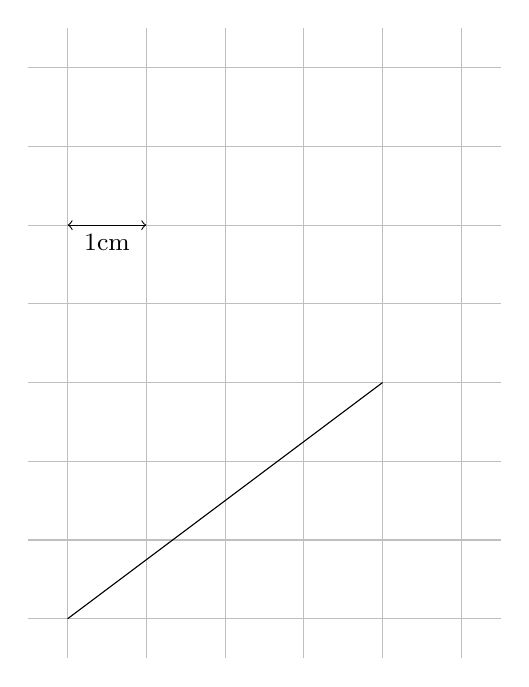
\begin{tikzpicture}
        \draw[color=gray!50] (-0.5,-0.5) grid[step=1] (5.5,7.5) ;
        \draw[<->] (0,5) -- node[below] {{\small \tunit{1}{cm}}} (1,5) ;
        \draw (0,0) -- (4,3) ;
    \end{tikzpicture}

    \task ~\\
    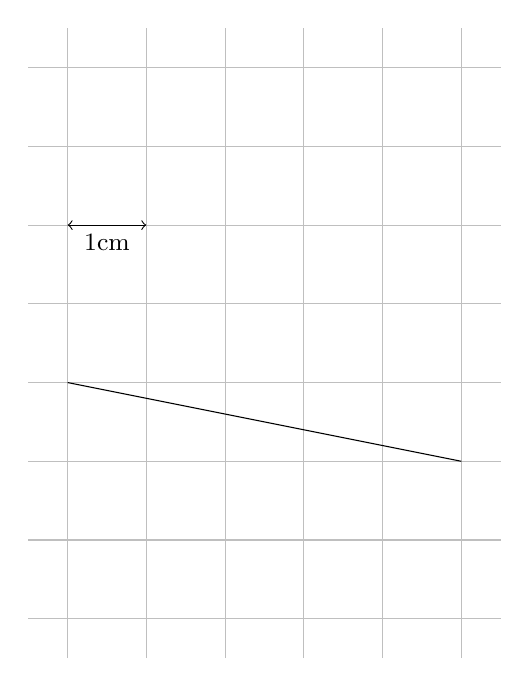
\begin{tikzpicture}
        \draw[color=gray!50] (-0.5,-0.5) grid[step=1] (5.5,7.5) ;
        \draw[<->] (0,5) -- node[below] {{\small \tunit{1}{cm}}} (1,5) ;
        \draw (0,3) -- (5,2) ;
    \end{tikzpicture}

    
    \task ~\\
    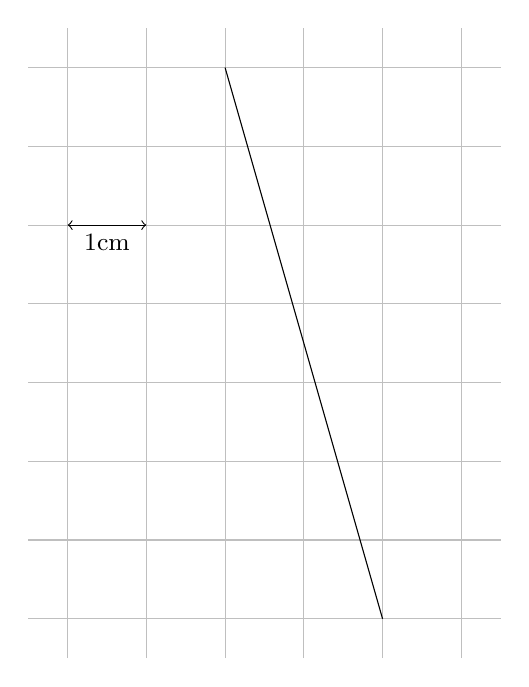
\begin{tikzpicture}
        \draw[color=gray!50] (-0.5,-0.5) grid[step=1] (5.5,7.5) ;
        \draw[<->] (0,5) -- node[below] {{\small \tunit{1}{cm}}} (1,5) ;
        \draw (2,7) -- (4,0) ;
    \end{tikzpicture}

    \task ~\\
    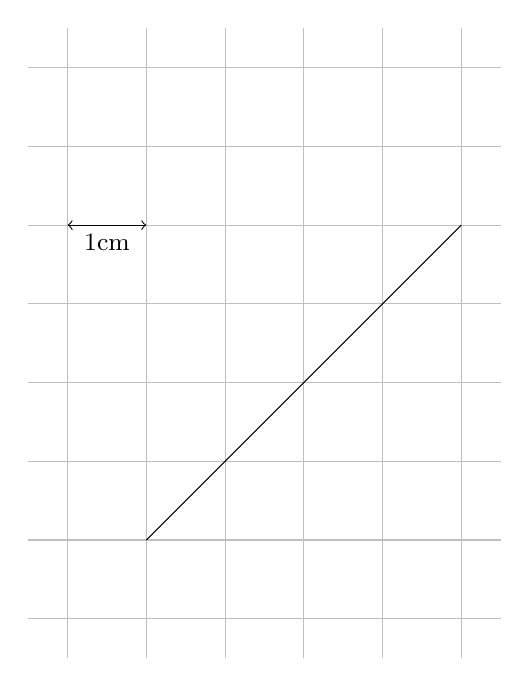
\begin{tikzpicture}
        \draw[color=gray!50] (-0.5,-0.5) grid[step=1] (5.5,7.5) ;
        \draw[<->] (0,5) -- node[below] {{\small \tunit{1}{cm}}} (1,5) ;
        \draw (1,1) -- (5,5) ;
    \end{tikzpicture}
\end{tasks}
}{1}    
\end{exop}


\begin{exo}{
Dessine les pentes.

\begin{tasks}(4)
    \task $40\%$
    \task $70\%$
    \task $100\%$
    \task $300\%$
\end{tasks}
}{1}    
\end{exo}

\begin{exo}{
Dessine les pentes.
\begin{tasks}(4)
    \task $\dfrac{1}{7}$
    \task $\dfrac{2}{3}$
    \task $2$
    \task $\dfrac{3}{2}$
\end{tasks}
}{1}    
\end{exo}

% Trouver la pente

\begin{exo}{
    Quelle est la pente d'une piste de ski si sa dénivellation est de \tunit{2}{m} et la distance horizontale correspondante de \tunit{5}{m} ?
}{1}
\end{exo}


\begin{exo}{
    Un poteau de \tunit{6}{m} projette une ombre de \tunit{10}{m} sur le sol. Quelle est la pente des rayons solaires ?
}{1}
\end{exo}




\begin{exo}{
    Voici quelques informations au sujet du funiculaire de Fribourg :
    \begin{itemize}
        \item Année de mise en service : $1899$
        \item Point bas : Neuveville, altitude \tunit{552,1}{m}
        \item Point haut : Saint-Pierre, altitude \tunit{608,5}{m}
        \item Longueur de la ligne \tunit{121}{m}
        \item Pente maximale $550$\textperthousand
    \end{itemize}
    Calcule la pente moyenne du funiculaire.
}{2}    
\end{exo}

\begin{exo}{
La pyramide de Khéops a une hauteur de \tunit{137}{m} et une base carrée de côté \tunit{230}{m}. Quelle est la pente de la
pyramide ?
}{1}
\end{exo}


% Trouver la dénivellation

\begin{exo}{
    La pente d'un chemin de montagne est de $5\%$. Quelle est la dénivellation correspondant à une distance horizontale de \tunit{1000}{m} ?
}{1}
\end{exo}

\begin{exo}{
    Joëlle mesure \tunit{1,60}{m}. Elle projette une ombre de \tunit{3,20}{m}.
    À côté d'elle se trouve un arbre qui projette une ombre de \tunit{15}{m}.

    \begin{tasks}
        \task Quelle est la hauteur de cet arbre ?
        \task Quelle est la pente des rayons solaires ?
    \end{tasks}
    
}{1}    
\end{exo}


\begin{exo}{
Une télécabine relie le village de Charmey (\tunit{876}{m} d'altitude) à Vounetse (\tunit{1617}{m}) sur une distance de \tunit{3146}{m}.

Quelle est la pente moyenne de la télécabine ?
}{1}
\end{exo}



\begin{exo}{
Mira et Sebastian vont à Aqua Parc. Mira teste le grand toboggan qui a une
pente de $20\%$. Sebastian, quant à lui, souhaite
commencer en douceur et prend le toboggan bleu dont la pente vaut $14\%$. Les deux toboggans ont la même distance horizontale de \tunit{65}{m}. Combien de mètres sépareront Mira et Sebastian aux points de départ ?
}{1}    
\end{exo}


%Trouver distance horizontale

\begin{exo}{
    La tour du Lignon mesure \tunit{91}{m} de hauteur. En été, la pente des rayons solaires est d'environ $60\%$.
    
    Quelle est la mesure au sol de l'ombre de l'immeuble ?
}{1}
\end{exo}


\begin{exo}{
    Un câble est tendu du sommet d'un chapiteau jusqu'au sol à une inclinaison de $65\%$. Le mât du chapiteau atteint une hauteur de \tunit{18}{m}. À quelle distance au sol du pied du mât sera attaché le câble ?
}{1}
\end{exo}


\begin{exo}{
 La tour de Pise a une hauteur de \tunit{56}{m} (mesure perpendiculaire au sol). Elle incline de $7\%$ par rapport à la verticale. Quelle est la distance entre la base de la tour et l'aplomb de son sommet ?
}{1}
\end{exo}

\begin{exo}{
Arjun descend une piste de ski dont la pente moyenne est de $110\%$. La piste commence à \tunit{2603}{m} d'altitude et finit à \tunit{2346}{m}.

\begin{tasks}
    \task Quelle est la distance, à vol d'oiseau entre le début et la fin de la piste ?

    \task Pour la même dénivellation, quelle serait la distance horizontale si la piste n'avait qu'une pente de $70\%$ ?
\end{tasks}

}{1}    
\end{exo}

\begin{exo}{
Raoul et Valentino sont à Europapark dans l'une des attractions vedettes : le Silver Star. La première rampe a une pente moyenne de $307,77\%$. Le point le plus haut est à \tunit{73}{m} du sol, et le plus bas à \tunit{3}{m}.
Quelle est la distance horizontale entre ces deux points ?
}{1}
\end{exo}

\begin{exol}{FA73}{87}{1} % pente
\end{exol}

\begin{exol}{FA76}{87}{1} % pente + altitude
\end{exol}

\begin{exof}{FA74}{90}{1} % pente droite
\end{exof}

\begin{exol}{FA75}{87}{1} % pente + échelle
\end{exol}

\begin{exol}{FA77}{87}{1}
\end{exol}


\begin{exof}{FA89}{94}{1} % pente + échelle
\end{exof}

\begin{exo}{
    Le départ d'une piste de ski est à \tunit{2428}{m} et l'arrivée est à \tunit{1582}{m}. Sur une carte à l'échelle $1:\numprint{30000}$, la longueur horizontale représente \tunit{12}{cm}.

    Quelle est la pente moyenne de cette descente ?
}{3}
\end{exo}


\begin{exo}{
Quelle est la pente moyenne d'une colline de \tunit{108}{m} de hauteur, si un village situé à son sommet et un autre à sa base sont distants de \tunit{15}{cm} sur une carte au $1:\numprint{6000}$
}{3}
\end{exo}


\begin{exo}{
Un téléphérique relie deux stations dont l'une est à \tunit{580}{m} d'altitude. Sur une carte au $1:\numprint{25000}$, les deux stations sont distantes de \tunit{6,5}{m}.

Calcule l'altitude de l'autre station en sachant que le câble du téléphérique a une pente de $28\%$.
}{3}
\end{exo}

\begin{exo}{
La distance entre deux villages est de \tunit{15}{cm} sur une carte au $1:\numprint{10000}$. La pente moyenne étant de $18\%$, calcule l'altitude du village le plus élevé sachant que l'autre village est à une altitude de \tunit{950}{m}.
}{3}
\end{exo}


\begin{exo}{
Un escalier a une pente de $18\%$ et relie deux étages dont la différence de niveau est de \tunit{3,6}{m}. Sur la maquette de l'architecte, la longueur horizontale est de \tunit{50}{cm}. 

Calcule l'échelle de cette maquette.
}{3}
\end{exo}



\begin{exo}{
La ville de Genève est située à \tunit{375}{m} d'altitude. La ville de Lausanne est, elle, située à \tunit{526}{m} d'altitude.
Sur une carte à l'échelle $1:\numprint{400000}$, la distance à vol d'oiseau qui les sépare est de \tunit{13}{cm}.

Quelle est la pente entre ces deux villes ?

}{3}
\end{exo}








\end{document}
